\documentclass{article}
%\usepackage[english]{babel}%
\usepackage{graphicx}
\usepackage{tabulary}
\usepackage{tabularx}
\usepackage[table,xcdraw]{xcolor}
\usepackage{pdflscape}
\usepackage{lastpage}
\usepackage{multirow}
\usepackage{cancel}
\usepackage{amsmath}
\usepackage[table]{xcolor}
\usepackage{fixltx2e}
\usepackage[T1]{fontenc}
\usepackage[utf8]{inputenc}
\usepackage{ifthen}
\usepackage{fancyhdr}
\usepackage[document]{ragged2e}
\usepackage[margin=1in,top=1.2in,headheight=57pt,headsep=0.1in]
{geometry}
\usepackage{ifthen}
\usepackage{fancyhdr}
\everymath{\displaystyle}
\usepackage[document]{ragged2e}
\usepackage{fancyhdr}
\usepackage[table,xcdraw]{xcolor}
% If you use beamer only pass "xcolor=table" option, i.e. \documentclass[xcolor=table]{beamer}
\usepackage[normalem]{ulem}
\useunder{\uline}{\ul}{}
\everymath{\displaystyle}
\linespread{2}%controls the spacing between lines. Bigger fractions means crowded lines%
%\pagestyle{fancy}
%\usepackage[margin=1 in, top=1in, includefoot]{geometry}
%\everymath{\displaystyle}
\linespread{1.3}%controls the spacing between lines. Bigger fractions means crowded lines%
%\pagestyle{fancy}
\pagestyle{fancy}
\setlength{\headheight}{56.2pt}


\chead{\ifthenelse{\value{page}=1}{
\includegraphics[scale=0.3]{BassettCTCLogo}\\ \textbf \textbf Water Reuse and Recycle}}
\rhead{\ifthenelse{\value{page}=1}{Shabbir Basrai}{Shabbir Basrai}}
\lhead{\ifthenelse{\value{page}=1}{}{\textbf Water Reuse and Recycle}}


\cfoot{}
\lfoot{Page \thepage\ of \pageref{LastPage}}
\rfoot{Module 8}
\renewcommand{\headrulewidth}{2pt}
\renewcommand{\footrulewidth}{1pt}
\begin{document}

\textbf{A PARADIGM SHIFT IN PROGRESS}\\
Water shortage is the lack of adequate accessible water resources to meet water needs within a locality. More than 1.2 billion people lack access to clean drinking water (United Nations, 2017). For localities where access to drinking water is readily available, an issue that is not necessarily recognized at this time is the one-and-done scenario discussed earlier—that is, safe drinking water quality water is drawn from a tap and used for a variety of purposes and that is that. After being used, this water is poured down drains or flushed down toilets—out of sight and out of mind. But, a significant paradigm shift is beginning to occur. The idea of toilet-to-tap reuse is not palatable to many people, but we need water. We cannot live without water. Fortunately, we can clean used water and reuse it, a task that Mother Nature often can do for us naturally. We have no other choice. Regions where water is readily accessible today may not be able to brag about that in the future. Population growth, overuse, misuse, abuse, and other events and actions affect water use and have detrimental impacts on water quality. We need to change the one-and-done scenario to a one-and-redone scenario by using technology to purify used water. The use of advanced treatment and purification of used water (wastewater) to drinking water quality is a paradigm change in progress.\\


\textbf{ADVANCED TREATMENT OF WASTEWATER TO DRINKING WATER QUALITY}\\
Advanced technologies and processes used for wastewater treatment and purification provided at indirect potable reuse (IPR) plants varies (see Figure 11.3) but are typically focused on providing multiple barriers for the removal of pathogens and organics. Nitrogen and TDS removal is provided at some locations where necessary. Table 11.2 shows most of the indirect potable reuse projects that have been implemented in the United States. The table has been sorted according to the type of potable reuse application (i.e., direct aquifer injection, aquifer recharge with surface spreading, and surface water augmentation). The first five projects shown in this table are direct injection
projects that match the proposed HRSD concept. Water extracted from direct injection and surface spreading projects that recharge groundwater is not typically treated again prior to distribution into the potable water system; however, water from surface water augmentation projects is typically treated again at water treatment plants because of water treatment requirements stipulated by the USEPA’s Surface Water Treatment Rule (SWTR). For example, Fairfax County’s Griffith Water Treatment Plant provides coagulation, sedimentation, ozone oxidation, biological activated carbon filtration, and chlorine disinfection for water extracted from the Occoquan Reservoir that is augmented by the Upper Occoquan Service Authority’s indirect potable reuse plant.
As shown in Table 11.2, the treatment provided for indirect potable reuse projects is typically a combination of multiple barriers for the removal of pathogens and organics. Multiple barriers for pathogens are typically provided through a combination of coagulation, flocculation, sedimentation, lime clarification, filtration (granular or membrane), and disinfection (chlorine, ultraviolet, or ozone). Multiple barriers for organics removal are typically provided through a combination of advanced
treatment processes (e.g., reverse osmosis, granular activated carbon, ozone in combination biological activated carbon), although conventional treatment processes (e.g., coagulation, softening) also provide removal at some locations. All potable reuse plants listed in Table 11.2 include a robust organics removal process of granular activated carbon (GAC), granular media filtration (GMF), biological activated carbon (BAC), reverse osmosis (RO), microfiltration (MF), ultraviolet advanced oxidation process (UVAOP), membrane bioreactor (MBR), or soil aquifer treatment (SAT), which are effective barriers to bulk and trace organics and represent the backbone of the potable treatment process. SAT is the controlled application of wastewater to earthen basins in permeable soils at a rate typically measured in terms of meters of liquid per week. The purpose of a soil aquifer treatment system is to provide a receiver aquifer capable of accepting liquid intended to recharge shallow groundwater, and system design and operating criteria are developed to achieve that goal. However, there are several alternatives with respect to the utilization or final fate of the treated water (USEPA, 2006):\\
\begin{itemize}
\item Groundwater recharge
\item Recovery of treated water for subsequent reuse or discharge
\item Recharge of adjacent surface streams
\item Seasonal storage of treated water beneath the site with seasonal recovery for agriculture
\end{itemize}
The SAT process typically includes application of the reclaimed water using spreading basins and subsequent percolation through the vadose zone. SAT provides significant removal of both pathogens and organics through biological activity and natural filtration. However, because some aquifers are confined, it is not possible to utilize the SAT for treatment through the vadose zone to recharge them. On the other hand, movement of reclaimed water through the aquifer after direct injection will provide significant treatment benefits, including excellent removal of pathogens. Advanced water treatment plants based on reverse osmosis and granular activated carbon are often utilized at locations where SAT treatment through the vadose zone is not feasible, because it is possible for these processes to be implemented at most locations.\\

\begin{table}[]
\begin{tabular}{lllll}
Project                                                            & Type of Potable Reuse Application                              & Year & Capacity (mgd) & Advanced Treatment Processes                                       \\
Hueco Bolton Recharge Project; El Paso, TX                         & Groundwater recharge via direct injection and spreading basins & 1985 & 10             & Lime + GMF + ozone + BAC + C                                       \\
West Basin Water Recycling Plant; Carson, CA                       & Groundwater recharge via direct injection                      & 1993 & 12.5           & MF + RO + UVAOP                                                    \\
Scottsdale Water Campus; Scottsdale, AZ                            & Groundwater recharge via direct injection                      & 1999 & 20             & MF + RO + Cl                                                      \\
Los Alamitos Seawater Intrusion Barrier; Long Beach, CA            & Groundwater recharge via direct injection                      & 2006 & 3              & MF + RO + UV disinfection                                          \\
Groundwater Replenishment                                          & Groundwater recharge via direct injection and spreading basins & 2008 & 70             & MF + RO + UVAOP + SAT (spreading basins for a portion of the flow) \\
Montebello Forebay, Groundwater Recharge District, Los Angeles, CA & Groundwater recharge via spreading basins                      & 1962 & 44             & GMF + C                                                            \\
Chino Basin Groundwater Recharge Project; Chico, CA                & Groundwater recharge via spreading basins                      & 2007 & 18             & GMF + O$_2$ + SAT (spreading basins)                                 
\\
Hueco Bolton Recharge Project; El Paso, TX                         & Groundwater recharge via direct injection and spreading basins & 1985 & 10             & Lime + GMF + ozone + BAC + C                                       \\
West Basin Water Recycling Plant; Carson, CA                       & Groundwater recharge via direct injection                      & 1993 & 12.5           & MF + RO + UVAOP                                                    \\
Scottsdale Water Campus; Scottsdale, AZ                            & Groundwater recharge via direct injection                      & 1999 & 20             & MF + RO + Cl$_2$ \\
Los Alamitos Seawater Intrusion Barrier; Long Beach, CA            & Groundwater recharge via direct injection                      & 2006 & 3              & MF + RO + UV disinfection                                          \\
Groundwater Replenishment                                          & Groundwater recharge via direct injection and spreading basins & 2008 & 70             & MF + RO + UVAOP + SAT (spreading basins for a portion of the flow) \\
Montebello Forebay, Groundwater Recharge District, Los Angeles, CA & Groundwater recharge via spreading basins                      & 1962 & 44             & GMF + C                                                            \\
Chino Basin Groundwater Recharge Project; Chico, CA                & Groundwater recharge via spreading basins                      & 2007 & 18             & GMF + O$_2$ + SAT (spreading basins)
\end{tabular}
\end{table}
Potential Supply Sources for Reuse Water\\
Sewage is not the only supply of reuse water.  Selecting the proper supply source of reuse water should consider the type and location of the end use.  Aside from municipal sewage, there are several other sources that can be treated including, but not necessarily limited to, the following supplies:\\
\begin{enumerate}
\item Urban Dry Weather Runoff
\item Oil and Gas Operations Flowback/Produced Water
\item Industrial/Food Industry Process Wastewater
\item Farm Drainwater
\item Ship Ballast Water
\end{enumerate}
 
Urban Dry Weather Runoff\\
It doesn't rain often in Southern California, so have you ever wondered why there's still some flow of water in some of the storm drains and channels?  This is urban dry weather runoff and are generally considered to be constant flows... rain or shine.  Urban runoff is often the source of the most pollution and occurs year-round due to inefficient watering of landscaping, hosing down sidewalks and driveways, washing cars, etc.  Urban runoff often carries trash, fertilizers, sediment, oil, auto fluids, pet waste, bacteria, and other contaminants to the nearest waterbody untreated.\\  

Oil and Gas Operations Flowback/Produced Water\\
Hydraulic fracturing (commonly known as "fracking") is a process used to extract natural gas or oil from impermeable rock formations in the ground that lock in the oil and gas.  Large quantities of water, chemicals, and sand are blasted into these formations at high pressures to crack the rock and release the trapped gas and oil into the flow returned to the surface.  The flowback water contains a lot of contaminants at high levels.  Flow is relatively continuous as long as the process is in operation.  Often fracking occurs in remote areas where there are fossil fuel sources.  There are many environmental groups that protest fracking operations for various reasons, and it is relatively controversial.\\
 
Industrial/Food Industry Process Wastewater\\
The food industry often uses water for its industrial food processes and produce a relatively consistent flow of wastewater when the facility is in operation.  This industrial process water could be used for rinsing food or producing the product.  The wastewater from these industrial food processes is often high in organics, nutrients, salts, and solids.\\
 
Farm Drainwater\\
Farms use a lot of water to irrigate crops, and the water not absorbed into the ground is conveyed by drainage channels to a collection point (intentional or unintentional).  Farms also use fertilizers and potentially pesticides/insecticides on their crops as well, which contaminates the drain water.  Drain water is often higher in TDS because as water evaporates and the salt concentrates and is left behind.  Farm drain water is somewhat regular, but not continuous and depends on irrigation cycles used by the farm.  Farms often try to optimize the amount of water used to meet needs.\\
      
  
Ship Ballast Water\\
Cruise ships, large tankers, and bulk cargo carriers take on ballast water for stability as the ship travels on its journey until reaching the destination point and then discharges the ballast water at the next port of call.  The ballast water is essentially sea water that contains plants, animals, viruses, and other microorganisms from that location.  Ballast water often results in non-native, nuisance, and exotic species being introduced into the marine environment.  This can cause public health and environmental risks resulting in significant economic cost to water/power utilities, commercial/recreational fisheries, agriculture, and tourism.  Clearly because it is seawater, it is high in TDS reflecting the ocean water.\\

2.12 Comparison of Reuse Supply\\
Throughout the course, we are sticking along the theme of matching supplies with demand in regards quantity AND quality.  So when comparing the various sources of wastewater supply that could be treated to produce recycled water, what would be the most appropriate source?
The table below shows the typical levels of the major water quality constituents for the various supply sources.  The column in the far right is the desired treatment levels for recycled water.
  
 
Ideally, we'd like to use the wastewater supply source that most closely matches the levels needed to achieve recycled water quality.  Here are some considerations to keep in mind:
\begin{enumerate}
\item Quantity - If the demand is for a lot of reuse water, then low flow supplies may not meet the demand.
\item Quality - Certain water quality constituents are easier to remove/treat than others. 
\begin{itemize} 
\item Organics (BOD/COD) and solids (TSS) requires conventional treatment processes. 
\item Nutrients (N and P) requires more specialized treatment processes. 
\item Salts (TDS) requires even more advanced treatment processes, meaning more energy and cost.
\item Other Constituents that we discussed previously (chemicals, pesticides, insecticides, oil, etc.) are not identified in the table above, and some of those types of constituents are just as difficult to treat.
\end{itemize}  
\item Timing - Industrial processes are typically operational during working daytime hours.  Irrigation demand is generally at night to early morning.  
\item Location - Where is the wastewater being generated?  Where is the recycled water demand?  If the wastewater is generated a far distance away from where the recycled water demand is located, then it is likely not economically feasible as a supply source.  Farming operations generally occur in rural areas and may not be near any metropolitan urban areas that may use recycled water for landscape irrigation.\\
\end{enumerate}
Keeping that in mind (quantity, quality, timing, and location), it's no wonder that the best source of recycled water is municipal sewage!  Sewage is continuously flowing in high quantities.  \\
The quality of municipal sewage is relatively easier to treat to recycled water standards.  
\\Recycled water demand is often in urban areas where the sewage is generated and primarily for irrigation, which occurs generally at night, while sewage flows are on a diurnal pattern (peak flows in morning and evening; low flow at night).  
\\Equalization basins or storage reservoirs are needed to accommodate the different timing of supply and demand. 
Urban runoff is another good source of reuse water because it is located in urban areas where recycled water demand is located. \\ 
Treatment processes are able to treat urban runoff for reuse, and it's continuously flowing.  \\
The only downside is that there's not enough of it to meet demand, BUT we can still capture it and reuse it as another supply source! \\
 
Recycled Water Irrigation\\

The most common application for recycled water is irrigation for landscape or agricultural.  If you drive around different areas and start seeing purple pipe or purple signs, then that area is irrigated with recycled water! \\
  
If recycled water is available:\\
\begin{itemize}
\item Cities will use recycled water for irrigation of landscaping alongside roads and in center medians. 
\item Homeowners Associations (HOAs) will use recycled water to irrigate common areas at entrances, community areas, or parks.
\item Golf courses will use recycled water to irrigate all the grass.  Certain areas may still be irrigated with potable (drinking) water because the grass (typically used on golfing putting greens) are particularly sensitive to salinity (or TDS). 
\item Agricultural farmers will use recycled water to irrigate their crops.  Depending on the type of recycled water and level of treatment, there may be certain limitations as to where and what kinds of crops that recycled water can be used for irrigation.  Additionally, certain plants are more sensitive to salinity, chloride, and boron; irrigation will have to be managed more closely.
\end{itemize}
Irrigation Water Considerations\\
The main considerations when using recycled water for irrigation are:\\
\begin{itemize}
\item TDS toxicity
\item Sodium impermeability
\item N and P overgrowth
\item Boron toxicity
\item TSS clogging
\end{itemize}
 
One of the most significant uses of reclaimed wastewater
\begin{itemize}
\item Water needed for irrigation in some states accounts for >80\% of demand
\item Regulations and guidelines vary widely from state to state
\item Guidelines for food crop use (21 states) and non-food crop use (40 states)
 \end{itemize}
 
 
 
TDS Toxicity\\
TDS is a combination of multiple constituents that are gen  rally labeled as "salts" or "salinity."  \\
High salinity (TDS) in irrigation water is bad for plants.  To explain why, let's talk about something more relatable to us.  \\

Have you ever eaten something really salty and then felt bloated afterwards or the next day?  That's because salt retains water; the more salt in your body, the more water your body retains.  Similarly, when you irrigate the ground with high salinity water, you are introducing more salt into the soil.  \\

The soil will then want to retain more water.  This can cause issues for plants with roots in the ground that are also trying to take in that water from the soil.  The salty soil is essentially fighting against the root to keep the water.  \\

If really high in salinity, then the soil will actually draw water from the root/plant.\\  

If the roots cannot uptake water from the soil, then the plant will weaken, growth will be stunted, less production (i.e. less fruit), more susceptible to poor weather, more susceptible to disease or pests, and may die.\\
  
Some of these constituents, particularly chloride (Cl), can be toxic to plants and cause leaf burn (yellowing/browning around the edges of leaves), which leads to reduced growth and productivity (i.e. production of fruits). \\

This can ultimately lead to excessive leaf drop.\\

Sodium Impermeability\\
While salinity is the presence of salts (or TDS), sodicity is the presence of sodium (Na+).  Sodium (Na+) is an ion with a strong ionic charge.  High levels of sodium can increase the SAR (sodium adsorption ratio).  As shown in the equation below, the SAR is essentially the ratio of sodium ion to the sum of calcium and magnesium ions.\\
 
Sodium ions (single positive charge) causes a weak attraction between soil particles, which generally have a slight negative charge on the surface. \\ Therefore, when using irrigation water with high sodium content, the soil will tend to break apart into smaller and smaller particles. \\ These small particles will seep a bit further down into the soil until it starts to buildup and over time form a clay layer. \\ Clay has very low permeability (i.e. does not allow water to pass through), therefore plant root systems will not want to grow very deep and will stay towards the surface (as shown in the figure below). \\ On the other hand, calcium and magnesium ions (double positive charge) result in a stronger attraction between soil particles and will want to keep the soil particles together (i.e. not flake off and form a clay layer). \\ This allows small channels in the ground for water to permeate to promote deeper root growth, which increases a plant's resiliency to changes in weather.\\
  
 
N and P Overgrowth\\
We've already discussed how nitrogen (N) and phosphorus (P) are essential nutrients for life and promote growth.  But as the saying goes, "Anything is excess is a poison."  High levels of N and P can cause excessive overgrowth either of the plant being grown or of other unintended growth like eutrophication and harmful algal blooms (HAB) with cyanobacteria toxins.   While nitrate can cause algal blooms too, phosphorus is often the limiting nutrient (i.e., the most scarce nutrient which limits growth) in aquatic ecosystems.  Increased available phosphorus has more of an impact to promote growth of algae than nitrogen.\\
   
Equally important on a regional scale, nitrate is soluble and gets transported easily in water. \\ High nitrates can be due to irrigation water, fertilizers, septic systems, wastewater treatment plants, dairies, and natural conditions. \\ Nitrate that is not used by the plants will continue to seep into the ground and make its way to the groundwater table where it may persist and accumulate for decades.  \\
Sensitive crops prefer irrigation water to have less than 5 mg/L N, which is typical of water recycling facilities capable of nitrification-denitrification (NDN).  More tolerant crops can handle higher levels of nitrogen and prefer less than 30 mg/L N.\\
This can lead to groundwater nitrate contamination.  Excessive nitrate in drinking water can adversely affect your health, particularly in babies it can result in methemoglobinemia (commonly known as blue baby syndrome).  Many agencies and joint efforts have implemented Salt and Nitrate Management Plans (SNMP) to protect the regional groundwater basins from contamination that is difficult to treat. The map of the United States below shows areas that are at the highest risk for nitrate contamination of shallow groundwaters.\\
 
Boron Toxicity\\
Boron (B) in high concentrations can also be toxic to plants, similar to chloride.  Boron can lead to chlorosis (yellowing of the leaf) which reduces growth, productivity, and may result in excessive leaf drop.\\ 
TSS Clogging\\
Irrigating the ground regularly with recycled water containing high levels of total suspended solids (TSS) can cause solid buildup and the small solids can clog the pores in the soil leading to less permeability for water to seep into the ground and be absorbed by the roots.  Often a clogging layer (less than 1/8 inch thick) may develop on the surface, which significantly reduces the permeability because it is almost like a thin layer of clay.  Have you ever seen a dried up lake bottom that looks like cracking (see picture below)?  This is the clogging layer that builds up over time.  Obviously, landscape irrigation is different from a lake, but it's a similar problem!\\
   
Source:  Orange County Water District. https://www.ocwd.com/news-events/newsletter/2017/august-2017/silt-removal-testing-shows-promise-to-maximize-percolation-rates-in-recharge-basins/  
 
Please select Next to move on to the next page.
  
2.14 Recycled Water Demands
The major demands for recycled water are:
\begin{itemize}
\item Irrigation
\item Pond/Lake Fill and Aquaculture
\item Cooling Towers
\item Industrial Uses (chip cleaning, boiler feed)
\item Fracking Water
\item Toilet Refilling
\item Aquifer Recharge (seawater barrier, potable)
\item Direct Potable Reuse
\end{itemize}

Pond/Lake Fill and Aquaculture\\
This is somewhat similar to irrigation. \\
The main considerations to use recycled water for ponds/lakes are:
\begin{itemize}
\item TDS Toxicity\\
\item N and P Overgrowth or Undergrowth - Need a balance of these essential nutrients.\\
\item Eutrophication causes Fish Kills and Odor\\
\item Excessive TSS Clogs Distribution System\\
\end{itemize}
Cooling Towers and Boilers
The main considerations to use recycled water for cooling towers and boilers are:
\begin{itemize}
\item TDS and Chloride Corrosion - Concentration of dissolved solids (which occurs in cooling towers and boilers due to evaporation) can cause corrosion.
\item Silica and Hardness Scaling - Buildup of silica or hardness inside the cooling tower or boiler will reduce the operating efficiency of the cooling tower or boiler. A layer of scale buildup as thin as 1/64 inch can reduce heat exchanger efficiency by 15\%.  It would require more energy, more blowdowns (drainage of water and replacement with fresh water), and more cost to operate.
\item Pathogens - Microbial growth inside these systems could also result in corrosion or scaling.  
\end{itemize}
Fracking Water\\
This is somewhat similar to cooling tower and boiler feed.  The main considerations to use recycled water for fracking are:
\begin{itemize}
\item TSS and Bacterial Growth leading to clogging
\item Hardness Scaling
\item Corrosion and Density Balance
\end{itemize}

Title 22 of California’s Code of Regulations refers to state guidelines for how treated and recycled water is discharged and used.\\

State discharge standards for recycled water and its reuse are regulated by the 1969 Porter-Cologne Water Quality Control Act and the State Water Resources Control Board’s 2019 Water Recycling Policy.\\

Title 22 lists 40 specific uses allowed with disinfected tertiary recycled water (such as irrigating parks), 24 specific uses allowed with disinfected secondary recycled water (such as irrigating animal feed and other unprocessed crops), and seven specific uses allowed with undisinfected secondary recycled water (such industrial uses).\\

Other allowed uses of the disinfected recycled water include irrigation of food crops and residential landscaping, supply of recreational impoundments for unrestricted body contact, air conditioning, commercial laundry, decorative fountains, and flushing toilets in commercial buildings.\\

The State Water Board governs the permitting of recycled water projects, develops uniform water recycling criteria and reviews and approves Title 22 engineering reports for recycled water use.\\

Wastewater treatment standards are set and enforced by the state’s nine regional water quality control boards in consultation with the California Department of Public Health. The nine regional boards are part of the State Water Board.\\

The State Water Board is reviewing recycled water use permits issued prior to Jan.1, 2001 to ensure consistency with all applicable regulations, including Title 22. If necessary, the State Water Board may require a new or updated Title 22 engineering report to be submitted for review and approval.\\

As part of its long-term planning, the state of California aims to:\\

Increase the use of recycled water over 2002 levels by at least 1 million acre-feet per year by 2020, and by at least 2 million acre-feet a year by 2030.\\
Increase the use of stormwater over 2007 levels by at least 500,000 acre-feet a year by 2020, and by at least 1 million acre-feet a year by 2030.\\

Water reuse involves using water more than once to expand a community’s available water supply.\\ The practice of water reuse occurs in various forms throughout the world. The latest advances in water technology allows for communities to reuse water for beneficial purposes including drinking, irrigation, and industrial processes. \\
The following terms are commonly used to describe the types and purposes of water reuse:
\begin{itemize}
\item Recycled or reclaimed water indicates water that has been used more than once.
\item De facto reuse occurs when downstream communities use surface water as a drinking water source that has been subjected to upstream wastewater discharges.
\item Nonpotable reuse refers to recycled or reclaimed water that is not used for drinking but is safe to use for irrigation or industrial processes.
\item Potable reuse refers to recycled or reclaimed water that is safe for drinking.
\end{itemize}
Advanced purification processes are proven technologies that transform treated wastewater into high-quality water—or purified water for potable reuse. \\
Purified water surpasses state and federal drinking water standards as well as additional water quality objectives. \\
In general, nonpotable reuse does not involve treatment to drinking water standards, and water quality objectives may vary depending on the end use and risk for human exposure. \\
Both potable and nonpotable reuse are practiced in the United States, and de facto reuse is relatively common.\\

Direct vs. Indirect Potable Reuse\\

In general, there are two forms of potable reuse:
\begin{enumerate}
\item Indirect potable reuse (IPR) introduces purified water into an environmental buffer (e.g., a groundwater aquifer or a surface water reservoir, lake, or river) before the blended water is introduced into a water supply system.
\item Direct potable reuse (DPR) introduces purified water directly into an existing water supply system.
\end{enumerate}
Many IPR projects have been established in the United States, and generally, they involve using reclaimed water to recharge groundwater aquifers and augment surface water reservoirs that are used as drinking water supplies.\\

There are two different approaches to implementing DPR. Both apply additional advanced treatment to the used water; however, the two differ in the location of blending. 
\begin{enumerate}
\item Here the purified water is blended with the raw water supplies (e.g., surface water or groundwater) before undergoing additional treatment process in a drinking water plant; 
\item This approach involves blending the purified water directly into the potable water distribution system downstream of the drinking water plant (i.e., pipe-to-pipe or direct-to-distribution DPR).
\end{enumerate}
Although both DPR and IPR provide significant additions to local water sup- plies, neither can meet all potable water demands.\\

To maximize resources, water managers often consider a diverse portfolio of water sources in their long-term strategy. Public water supplies in North America come from various sources including surface water, ground- water, desalinated seawater and brackish groundwater, and reused water. \\
Planning and managing water resources becomes increasingly complex as surface water and groundwater supplies in many regions are stressed. \\
Additionally, desalination of seawater or brackish ground- water is not always economically feasible.\\
Importing water from other communities has a high price tag as well. As a result, many communities are incorporating potable reuse into their integrated water resources plan as a practical solution to ensure reliable water sources for the future. \\
Potable reuse offers many benefits in addition to playing an integral role in a water portfolio.\\


\textbf{What are the benefits of potable reuse?}\\

Because potable reuse provides especially high-quality water, the end-uses are more diverse than for other types of reclaimed water. \\
For example, in addition to drinking water, applications include agricultural and landscape irrigation, industrial processes, and other municipal uses. \\
Environmentally, potable reuse is a more sustainable water supply, making more efficient use of existing water supplies by recycling a resource that would otherwise be discharged.\\
Potable reuse may:
\begin{itemize}
\item  Decrease the amount of water imported to urban areas (in many cases, from long distances), 
\item Reduce groundwater extraction, and minimize wastewater discharges to the environment. \\
\begin{itemize}
\item Energy costs are lowered
\item Groundwater overdrafts are limited, and 
\item Health of aquatic ecosystems that receive wastewater effluent is improved.
\end{itemize}
\item potable reuse utilizes a local resource that is accessible for many water systems throughout the country, unlike sources such as seawater and brackish groundwater, which may not be available depending on geography and geology.
\end{itemize}
Is potable reuse regulated?\\
Federal potable reuse regulations have not been developed in the United States. \\
Thus, state and local agencies are responsible for setting potable reuse standards. The majority of states have established regulations or guidelines for water reuse (Figure 5. www.awwa.org/reuse), and state regulations are expected to be regularly updated and developed as states gain experience and confidence in water reuse. \\
Although few states have established regulations or guidelines specifically for potable reuse, most will still consider potable reuse projects on a case-by-case basis. \\
A summary of each state’s water reuse requirements (not specific to potable reuse) is provided in the US Environmental Protection Agency (USEPA) document Guidelines for Water Reuse (2012), along with recommendations for water reuse opportunities, technical guidance, and key considerations for implementing reuse projects.\\
Additionally, in a collaborative effort, the WateReuse Research Foundation, the American Water Works Association, Water Environment Federation, and National Water Research Institute developed a framework for DPR.\\
This framework document provides information about the value of DPR as a water supply option and the fundamental components to implementing a DPR program (Figure 6).\\

Regardless of the source, all potable water distributed to communities meets drinking water quality standards derived from the Safe Drinking Water Act (SDWA). \\
Established in 1974, the SDWA provides the framework for USEPA to set the minimum quality standards for drinking water and requires all public water suppliers to comply with those standards.\\ 
However, source water for potable reuse is also regulated further upstream. \\
The Clean Water Act (CWA), established in 1972, regulates pollutant discharges and allows USEPA to set quality standards for surface waters in the United States. \\
The CWA was integral for protecting and improving the quality of source waters throughout the nation, thereby making potable water reuse attainable. Building on these two critical pieces of legislation, the water industry can utilize potable reuse to augment public water sup- plies in a manner that is protective of public health.
Potable reuse is also growing in popularity in both Canada and Mexico, although specific potable re- use regulations have not been developed in either country. However, potable reuse projects are considered on a case-by-case basis where appropriate.\\
\textbf{Public Health Protection}\\
Public health protection is at the forefront of potable reuse. \\
Considering the multitude of people who rely on public drinking water supplies, ensuring public health and safety is of utmost importance to water professionals. \\
A wide range of established treatment options and process combinations are available to ensure that potable reuse produces the best water quality that protects against adverse health effects from contaminant exposure. \\
Public health concerns are a driving force to advance research efforts, develop new regulations, enhance treatment technologies, and train skilled water operators

\textbf{Potable Reuse Treatment}\\
There are as many as four different treatment points associated with potable reuse.\\
\begin{enumerate}
\item All wastewater is treated prior to discharge using one or more of the following steps:
\begin{enumerate}
\item Preliminary Treatment—Removal of suspended and floating particles that may cause operational or maintenance problems with subsequent treatment processes
\item Primary Treatment—Removal of a portion of the suspended solids and organic matter
\item Secondary Treatment—Removal of most of the sus- pended solids and organic matter
\item Tertiary Treatment—Removal of targeted dissolved solids and finer suspended materials
\end{enumerate}
\item Advanced Treatment-The treated wastewater becomes the source of supply for potable reuse, which uses a combination of advanced processes in a second point of treatment.\\ 
Advanced Treatment may include one or more of the following processes in combination to not only achieve water quality goals, but also provide resilient, redundant, and robust treatment in a multiple barrier approach to contaminant removal.
\begin{itemize}
\item Biological Treatment—The use of bacteria and other microorganisms to consume and remove or- ganic materials and nutrients in the water; examples include biologically active media filters and anaerobic denitrifying filters (specifically for the removal of nitrate and nitrite).
\item Membrane Filtration—Processes that use a membrane barrier with microscopic pores to remove suspended particles and pathogenic microorganisms; examples include microfiltration (MF) and ultrafiltra- tion (UF).
\item Membrane Desalination—Processes that use a non-porous, semipermeable membrane barrier to remove salts, pharmaceuticals, and other dissolved contaminants; examples include reverse osmosis (RO) and nanofiltration (NF).
\item Ozone—A powerful oxidant used for disinfection and/or breaking down organic contaminants, includ- ing pharmaceuticals.
\item Advanced Oxidation—Processes used to achieve significant pathogen disinfection and break down organic contaminants, including pharmaceuticals; examples include ozone (O3) or ultraviolet (UV) light in combination with hydrogen peroxide.
\end{itemize}
\item In addition to the wastewater and advanced potable re- use treatment described above, IPR also uses an environmental buffer either before or after advanced treatment  as a third point of treatment. 
\begin{itemize}
\item The environmental buffer may be a groundwater aquifer, surface water reservoir, or even natural or constructed wetlands, providing storage, hydraulic transport, and/or an additional barrier for the protection of public health.\\
Although DPR does not include an environmental barrier, it does use an engineered storage buffer. 
\begin{itemize}
\item If the DPR approach involves blending the purified water with the raw water supplies prior to a subsequent drinking water plant, the engineered storage buffer occurs between the advanced and drink- ing water treatment plants. 
\item For pipe-to-pipe DPR, the engineered storage buffer occurs between the advanced treatment plant and potable water distribution system.
\end{itemize}
\end{itemize}
\item Missing
\end{enumerate}

Potable reuse – Recycled or reclaimed water that is safe for drinking.  There are two types of potable reuse:  indirect and direct. 
\begin{enumerate} 
\item Indirect Potable Reuse (IPR) - The planned incorporation of reclaimed water into a raw water supply such as in potable water storage reservoirs or a groundwater aquifer, resulting in mixing and assimilation, thus providing an environmental buffer.
\item Direct Potable Reuse (DPR) - The introduction of highly treated reclaimed water either directly into the potable water supply distribution system downstream of a water treatment plant, or into the raw water supply immediately upstream of a water treatment plant.
\end{enumerate}

While the terms IPR and DPR are still used, there is a transition in terminology to be more specific about the type of potable reuse:
\begin{itemize}
\item Groundwater augmentation (GWA) - Advanced treated water is recharged/injected into the groundwater basin used as a water supply.
\item Surface (reservoir) water augmentation (SWA) - Advanced treated water (+) is discharged into a surface reservoir used as raw water supply. 
\item Raw water augmentation (RWA) - Advanced treated water (++) is discharged directly upstream of a drinking water treatment plant.
\item Treated water augmentation (TWA) - Advanced treated water (+++) is discharged downstream of the drinking water treatment plant directly into the potable water distribution system.
\end{itemize}

State of California, Title 22 Code of Regulations (Links to an external site.) (Title 22, CCR) identifies multiple specific end uses allowed for the different types of recycled water.  Here are a few examples of end uses:
\begin{itemize}
\item Irrigation of parks, animal feed, other unprocessed crops, food crops, residential landscaping, supply of recreational impoundments for unrestricted body contact
\item Air conditioning
\item Commercial laundry
\item Decorative fountains
\item Flushing toilets in commercial buildings
\item Industrial processes
\item Environmental restoration
\item Groundwater Augmentation (GWA)
\item Surface Water Augmentation (SWA) [recently added]
\end{itemize}



\begin{figure}
\begin{center}
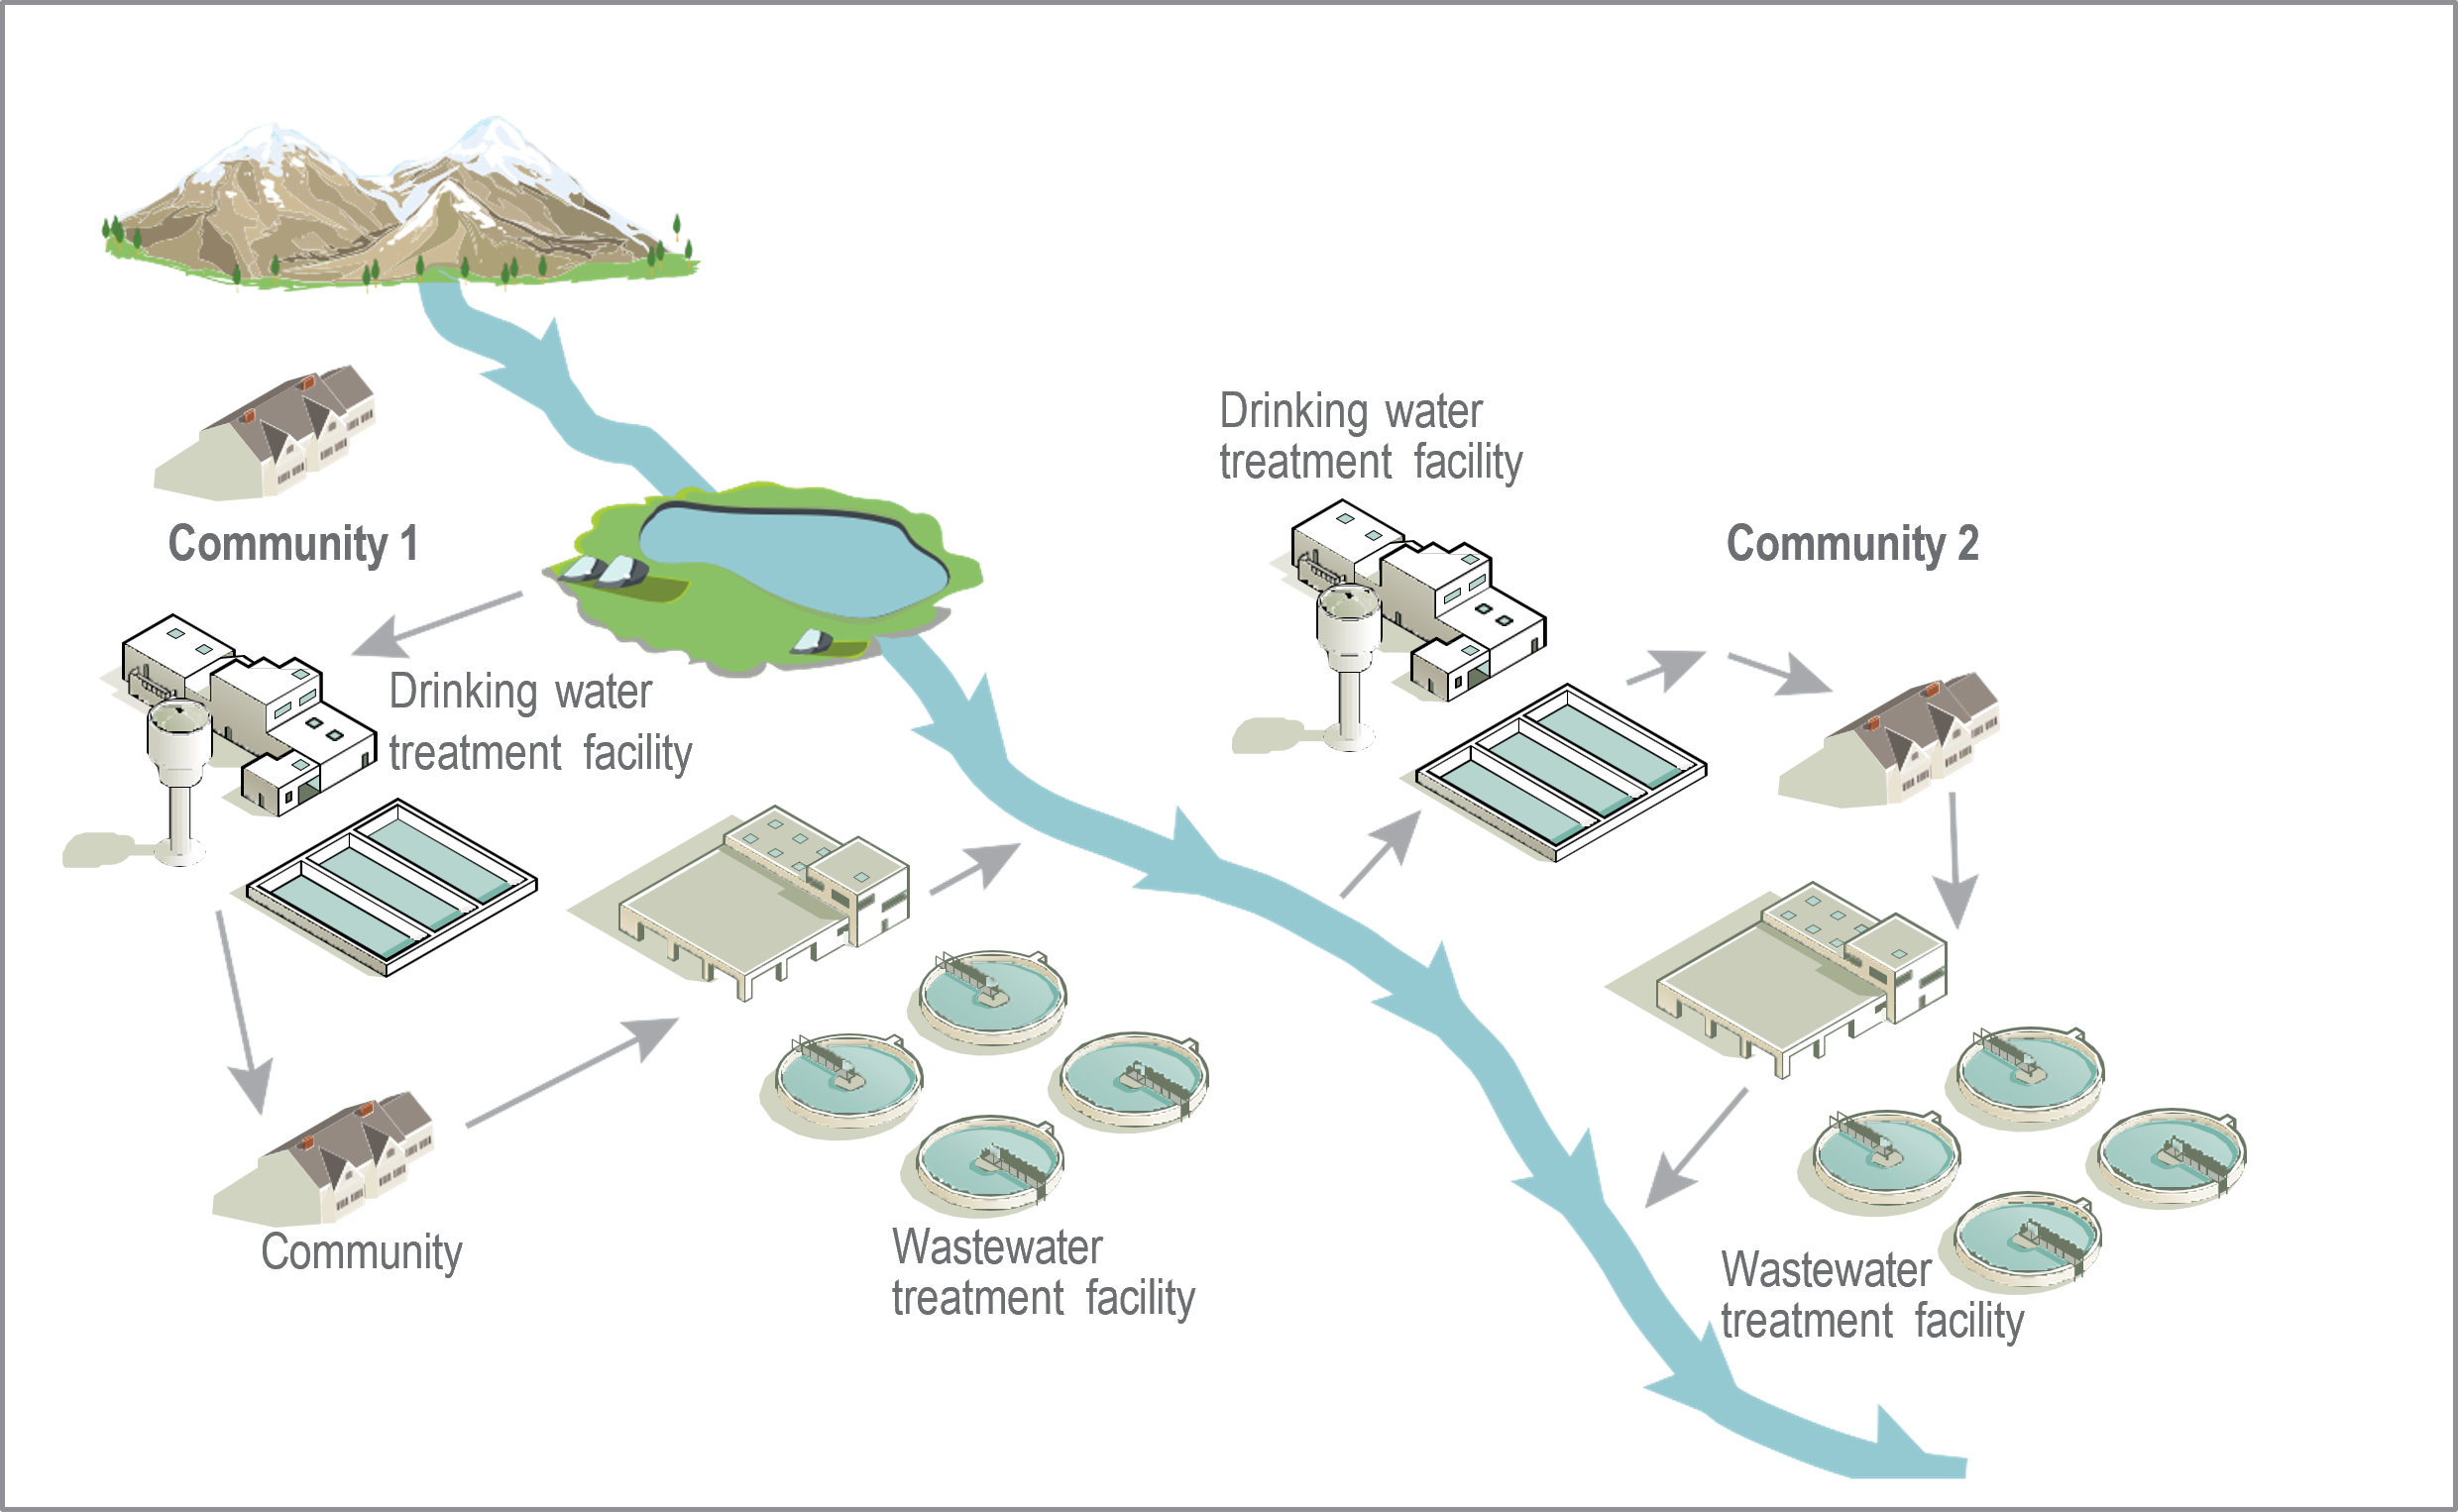
\includegraphics[scale=0.8]{DefactoWaterReuse}
\caption{De-facto Water Reuse Flow Schematic}
\end{center}
\end{figure}


\begin{figure}
\begin{center}
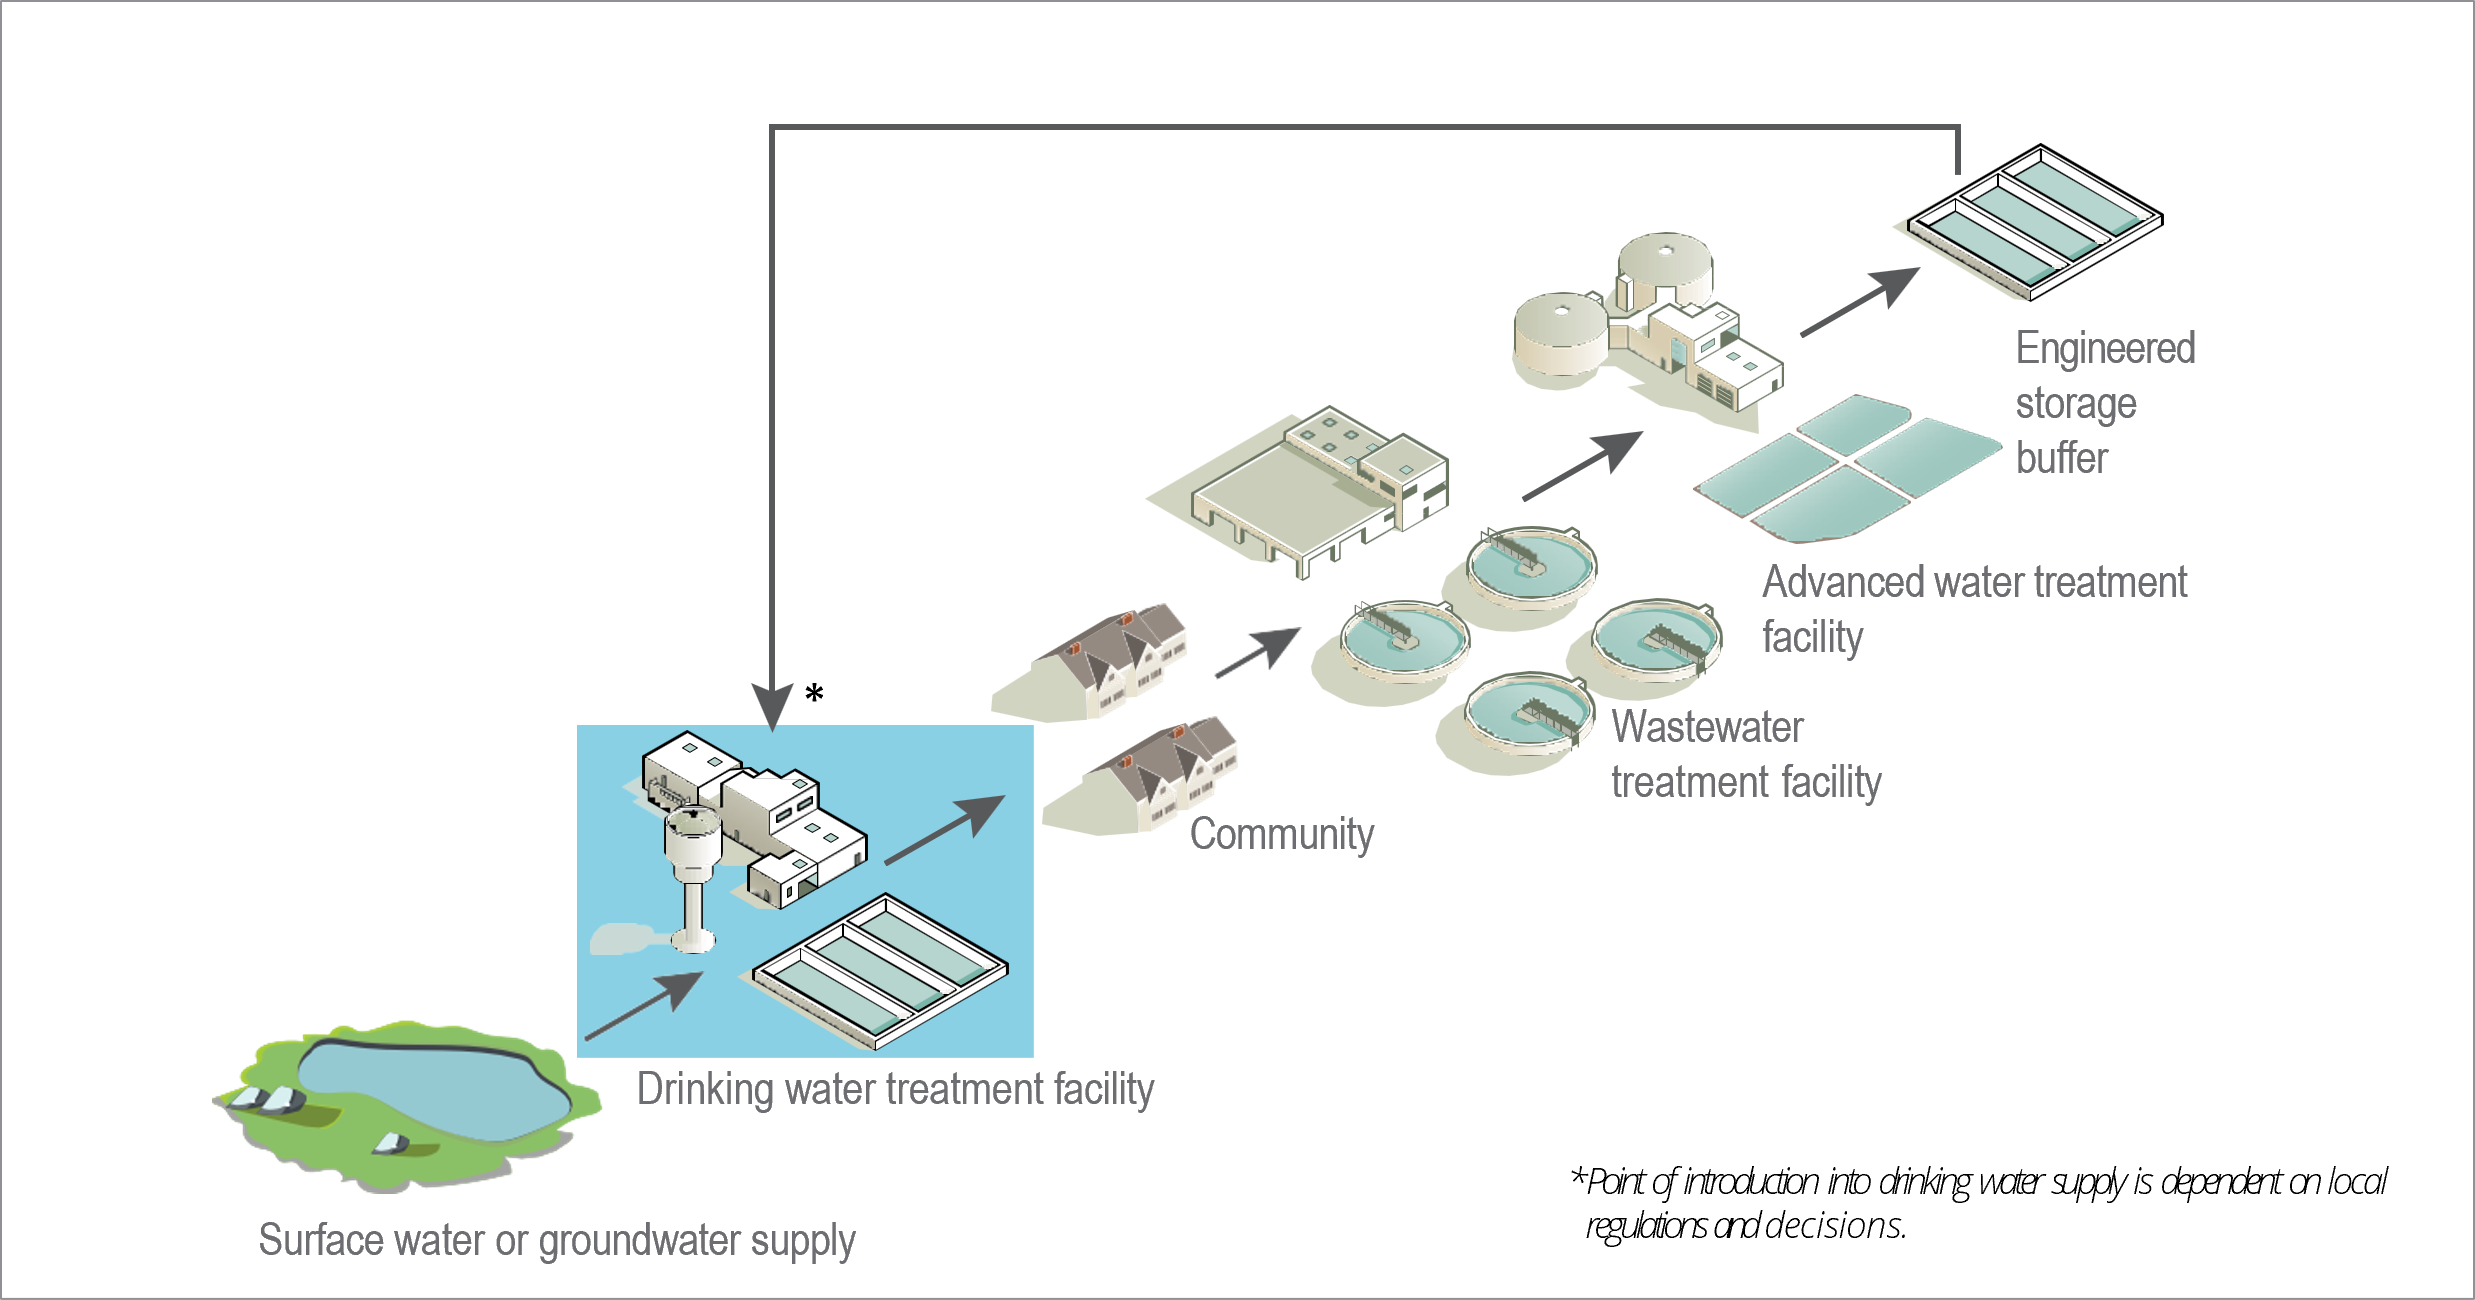
\includegraphics[scale=0.8]{DirectPotableReuse}
\caption{Direct Potable Reuse Flow Schematic}
\end{center}
\end{figure}

\begin{figure}
\begin{center}
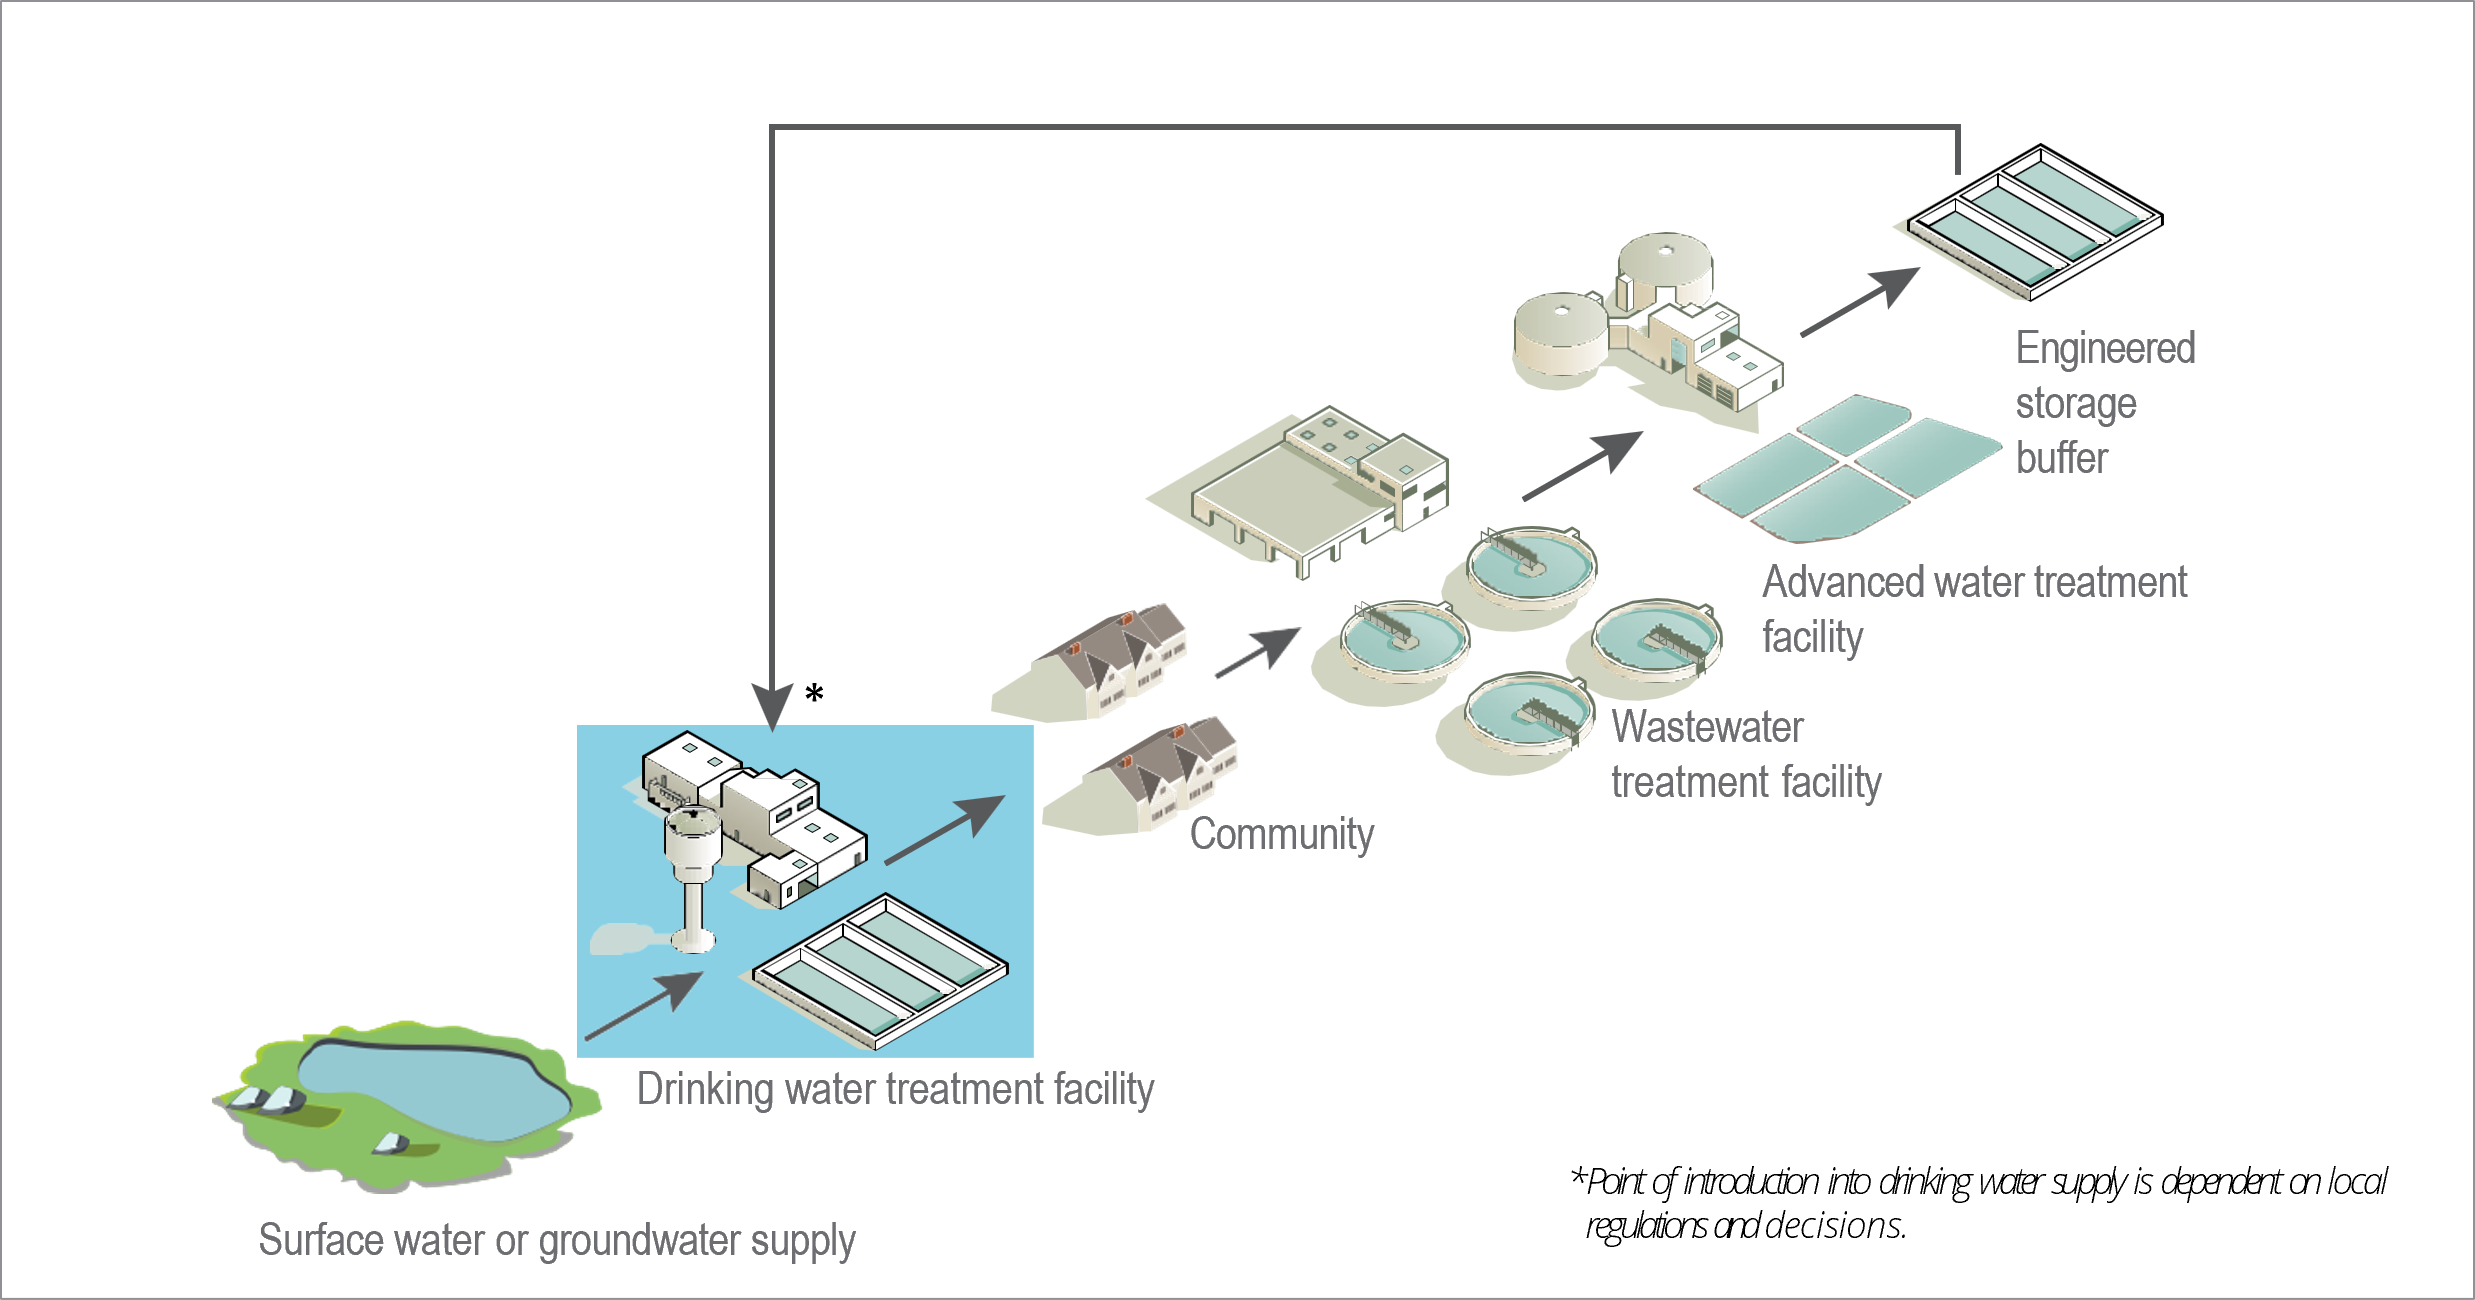
\includegraphics[scale=0.8]{DirectPotableReuse}
\caption{Indirect Potable Reuse Flow Schematic}
\end{center}
\end{figure}
\end{document}